
\documentclass[a4paper,11pt]{article}%,twocolumn
%% packages

\usepackage{blindtext} % needed for creating dummy text passages
%\usepackage{ngerman} % needed for German default language
\usepackage{amsmath} % needed for command eqref
\usepackage{amssymb} % needed for math fonts
\usepackage[colorlinks=true,breaklinks]{hyperref} % needed for creating hyperlinks in the document, the option colorlinks=true gets rid of the awful boxes, breaklinks breaks lonkg links (list of figures), and ngerman sets everything for german as default hyperlinks language
\usepackage[hyphenbreaks]{breakurl} % ben�tigt f�r das Brechen von URLs in Literaturreferenzen, hyphenbreaks auch bei links, die �ber eine Seite gehen (mit hyphenation).
\usepackage{xcolor}
\definecolor{c1}{rgb}{0,0,1} % blue
\definecolor{c2}{rgb}{0,0.3,0.9} % light blue
\definecolor{c3}{rgb}{0.3,0,0.9} % red blue
\hypersetup{
    linkcolor={c1}, % internal links
    citecolor={c2}, % citations
    urlcolor={c3} % external links/urls
}
%\usepackage{cite} % needed for cite
\usepackage[square,authoryear]{natbib} % needed for cite and abbrvnat bibliography style
\usepackage[nottoc]{tocbibind} % needed for displaying bibliography and other in the table of contents
\usepackage{graphicx} % needed for \includegraphics 
\usepackage{longtable} % needed for long tables over pages
\usepackage{bigstrut} % needed for the command \bigstrut
\usepackage{enumerate} % needed for some options in enumerate
%\usepackage{todonotes} % needed for todos
\usepackage{makeidx} % needed for creating an index
\makeindex
\usepackage{gensymb}
\usepackage{url}
\usepackage{psfrag}
\usepackage{multirow}
\usepackage{subfigure}
%% page settings

\usepackage[top=20mm, bottom=20mm,left=15mm,right=15mm]{geometry} % needed for page border settings
\parindent=0mm % for space of first line of new text block
\sloppy % for writing with hyphenless justification (tries to)
\hyphenation{} % use hyphenation of tolerance parametershttp://www.jr-x.de/publikationen/latex/tipps/zeilenumbruch.html
\hyphenpenalty=10000
\exhyphenpenalty=10000
\usepackage{fancyhdr} % needed for head and foot options
%% my macros

%% Text fomats
\newcommand{\tbi}[1]{\textbf{\textit{#1}}}

%% Math fonts
\newcommand{\bbA}{\mathbb{A}}
\newcommand{\bbB}{\mathbb{B}}
\newcommand{\bbC}{\mathbb{C}}
\newcommand{\bbD}{\mathbb{D}}
\newcommand{\bbE}{\mathbb{E}}
\newcommand{\bbF}{\mathbb{F}}
\newcommand{\bbG}{\mathbb{G}}
\newcommand{\bbH}{\mathbb{H}}
\newcommand{\bbI}{\mathbb{I}}
\newcommand{\bbJ}{\mathbb{J}}
\newcommand{\bbK}{\mathbb{K}}
\newcommand{\bbL}{\mathbb{L}}
\newcommand{\bbM}{\mathbb{M}}
\newcommand{\bbN}{\mathbb{N}}
\newcommand{\bbO}{\mathbb{O}}
\newcommand{\bbP}{\mathbb{P}}
\newcommand{\bbQ}{\mathbb{Q}}
\newcommand{\bbR}{\mathbb{R}}
\newcommand{\bbS}{\mathbb{S}}
\newcommand{\bbT}{\mathbb{T}}
\newcommand{\bbU}{\mathbb{U}}
\newcommand{\bbV}{\mathbb{V}}
\newcommand{\bbW}{\mathbb{W}}
\newcommand{\bbX}{\mathbb{X}}
\newcommand{\bbY}{\mathbb{Y}}
\newcommand{\bbZ}{\mathbb{Z}}


% Define colors
\definecolor{codegreen}{rgb}{0,0.6,0}
\definecolor{codegray}{rgb}{0.5,0.5,0.5}
\definecolor{codepurple}{rgb}{0.58,0,0.82}
\definecolor{backcolour}{rgb}{0.95,0.95,0.92}
% Setup the listings package
\lstset{
    backgroundcolor=\color{backcolour},   
    commentstyle=\color{codegreen},
    keywordstyle=\color{magenta},
    numberstyle=\tiny\color{codegray},
    stringstyle=\color{codepurple},
    basicstyle=\footnotesize,
    breakatwhitespace=false,         
    breaklines=true,                 
    captionpos=b,                    
    keepspaces=true,                 
    numbers=left,                    
    numbersep=5pt,                  
    showspaces=false,                
    showstringspaces=false,
    showtabs=false,                  
    tabsize=2
}



\begin{document}
\begin{titlepage}
\center % Center everything on the page

%-------------------------------------------------------------------------------------
%	HEADING SECTIONS
%------------------------------------------------------------------------------------
\textbf{\large Department of Electrical and Computer Engineering}\\[0.5cm]
\textbf{\Large University of Colorado at Boulder}\\[1cm]
\textbf{\large ECEN5730 - Practical PCB design}\\[2cm]

\includegraphics[width=0.3\textwidth]{figures/cu}\\[2cm] 

	
%-------------------------------------------------------------------------------------
%	TITLE SECTION
%------------------------------------------------------------------------------------

\textbf{\Huge Board Good Layout/Bad Layout }\\[0.2cm]

\textbf{\Large Report}\\[2cm]
\vspace{1.5cm}
\begin{figure}[H]
	\centering
	
\includegraphics[scale=0.2]{figures/qr_download.png}
	\label{555_schematic}
\end{figure}\vspace{1.5cm}


%----------------------------------------------------------------------------------------
%	MEMBERS SECTION
%----------------------------------------------------------------------------------------


\vfill

\textbf{\large Submitted by}

{\large Parth Thakkar}\\[0.5cm]




%----------------------------------------------------------------------------------------
%	DATE SECTION
%----------------------------------------------------------------------------------------

\textbf{\large Submitted on}\\
\textbf{\Large \today} % Date, change the \today to a set date if you want to be precise

%----------------------------------------------------------------------------------------

\vfill % Fill the rest of the page with whitespace

\end{titlepage}

\pagebreak

\tableofcontents
\listoffigures
\listoftables
\vfill
\begin{center}
	\textbf{\textit{*PDF is clickable}}
\end{center}

\pagebreak

\section{Objective / Purpose of Lab}

This laboratory experiment goes into the critical role of printed circuit board (PCB) layout in reducing switching noise. The primary objective is to quantify and compare the switching noise generated by different layout practices on a dedicated test board(Prof. Bogatin's board).\\

The specifically designed test board comprises three distinct regions:

\begin{itemize}
	\item \textbf{Good Layout:} This region embodies optimal design principles, featuring a continuous return path beneath signal traces and decoupling capacitors strategically placed close to integrated circuit (IC) power pins.
	\item \textbf{Bad Layout 1:} Deliberately lacking a return path and employing distant decoupling capacitors, this region exemplifies poor design practices known to exacerbate switching noise.
	\item \textbf{Bad Layout 2:} While incorporating a return path, this region maintains the disadvantage of remote decoupling capacitors, creating a scenario with compromised noise performance.\\





\end{itemize}

By systematically analyzing the switching noise on each region, the following key objectives will be achieved:

\begin{itemize}
	\item Quantify the impact of layout practices on switching noise: This involves measuring and comparing the noise levels on critical signals, including quiet low (Q\_low), quiet high (Q\_hi), trigger output, and power rails (5V and 3.3V).
	\item Relate observed noise levels to specific design choices: Through analysis, the experiment aims to establish a clear connection between the noise behavior observed in each region and the corresponding layout features employed.
	\item Formulate practical recommendations for future designs: Based on the findings, the experiment seeks to establish valuable guidelines for minimizing switching noise in future PCB layouts.

\end{itemize}

This experiment holds significant relevance for aspiring and practicing electrical engineers, as it underscores the practical implications of theoretical design principles in achieving robust and reliable electronic circuits.\\

Here is the Prof. Eric Bogatin's board that we have to measure noise in.

\begin{figure}[H]
	\centering
	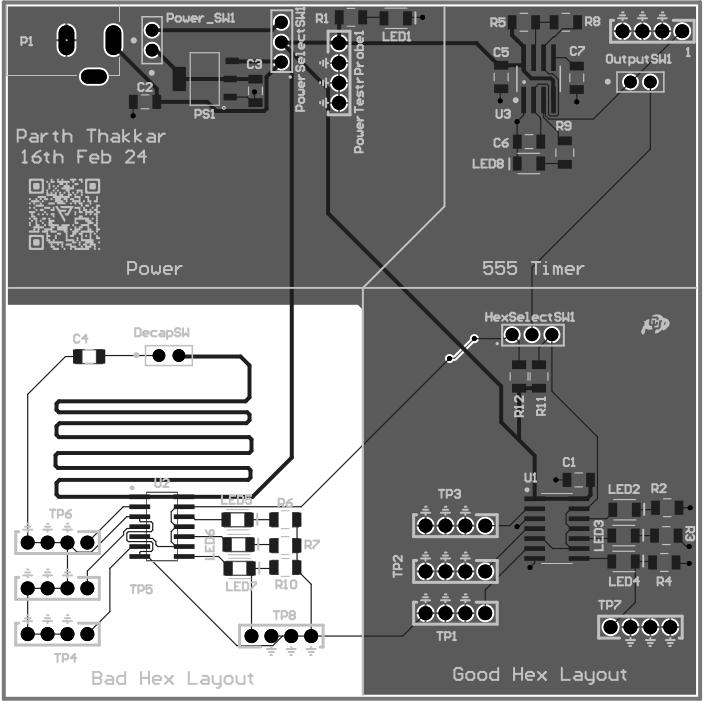
\includegraphics[scale=0.12]{figures/pcb}
	\caption{PCB}

\end{figure}

Here is the block diagram of the PCB
\begin{figure}[H]
	\centering
	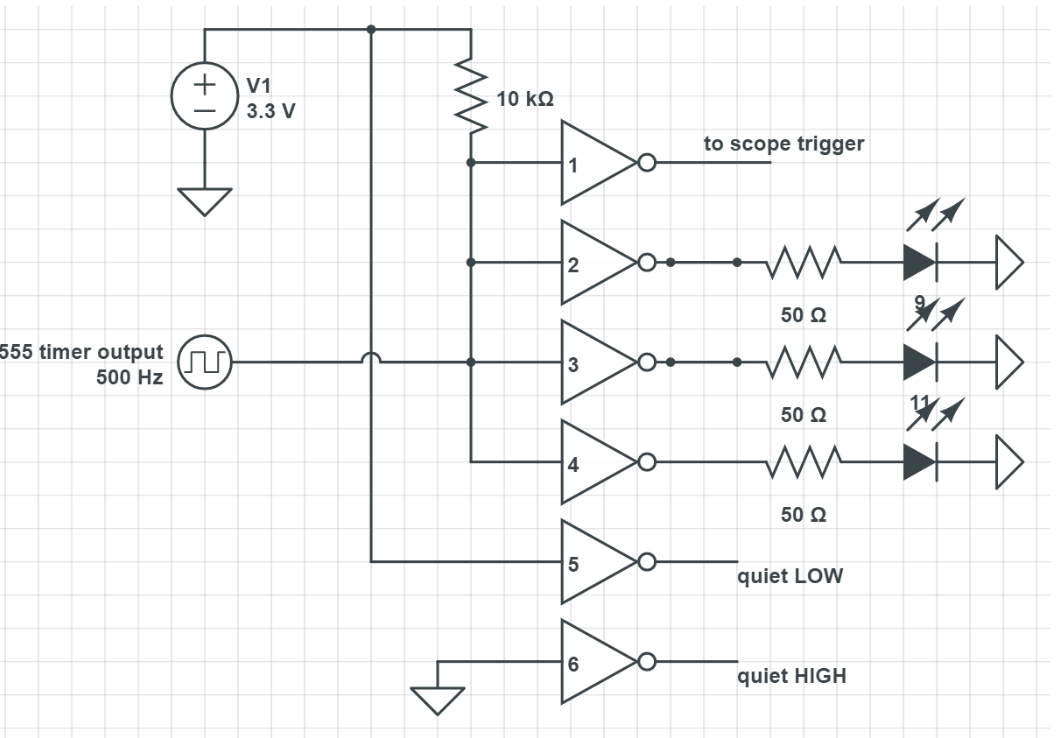
\includegraphics[scale=0.3]{figures/blockdiagram.png}
	\caption{PCB}

\end{figure}
\section{Component listing}


\begin{table}[H]
	\centering
	\begin{tabular}{|c|l|}
		\hline
		  & \textbf{Component Name}               \\\hline
		  &                                       \\
		1 & Digital Multimeter (DMM)              \\
		2 & Power Suppy                           \\
		3 & Test PCB of Professor Bogatin         \\
		4 & Cables and connectors for measurement \\
		\hline\hline
	\end{tabular}
	\caption{Component list}
	\label{filterspecs}
\end{table}





\section{Explanation}

\begin{itemize}
	\item \textbf{Switching Noise:} When digital circuits transition between logic states (high or low), rapid current changes occur. These rapid changes can induce unwanted voltage fluctuations on the power and ground planes, known as switching noise. This noise can couple into neighboring signals, causing errors and compromising circuit performance.
	\item Impact of Layout Practices:

	      \begin{itemize}
		      \item \textbf{Continuous Return Path:} A dedicated low-impedance path for current flow minimizes voltage drops and ground bounce during switching events.
		      \item \textbf{Decoupling Capacitors:} Placed close to IC power pins, these capacitors act as local energy storage, providing a readily available current source during switching and mitigating voltage fluctuations on the power plane.
		      \item \textbf{Trace Length and Width:} Shorter and wider traces offer lower resistance, minimizing voltage drops and associated noise generation.
	      \end{itemize}
	\item \textbf{Test Board Design:} The test board features a clock signal generated by a 555 timer, driving three separate hex inverter circuits. Each circuit resides in a dedicated region (good layout, bad layout 1, bad layout 2) to isolate the effects of layout choices.
\end{itemize}




\section{Procedure}


\textbf{Measurement Procedure:}
Good/Bad Layout Measurements:
\begin{itemize}
	\item Trigger the oscilloscope on the designated trigger output test point.
	Measure the rise and fall times of the trigger signal.
	\item Measure the voltage noise on the Q\_low and Q\_hi test points.
	Zoom in on the 5V and 3.3V rail test points to observe any synchronous noise with the switching signal.
	\item Repeat these measurements for all layouts, Bad layout1 and Bad layout 2
\end{itemize}



\section{Expected Outcomes}
\begin{itemize}
	\item 	Significantly lower noise levels in the good layout region compared to the bad layouts.
	\item A clear correlation between the presence of beneficial layout features (return path, close decoupling capacitors) and reduced switching noise.
	\item Valuable insights into the practical impact of layout practices on circuit performance.
\end{itemize}

\section{Calculations}

\textbf{Percentage Improvement:}

we can measure the improvement from the worst Layout to good layout and worst layout to bad layout from this formula\\


\begin{flalign*}
	&Percentage Improvement = \frac{Noise_{bad} - Noise_{good}} {Noise_{bad}} * 100 \% &&\\
	&Percentage Improvement = \frac{1.6884 - 0.220} {1.6884} * 100 \% &&\\
	&\boxed{Percentage Improvement = 86.99 \%}&&\\
\end{flalign*}


In our case we got around 87\% of noise improvement from bad layout to good layout

\section{Measurement}
\begin{enumerate}

	\item \textbf{Q\_low Noise:}

	\textbf{Measurement:} Measure the peak-to-peak voltage of the noise observed on the Q\_low test point using the oscilloscope.

	\begin{figure}[H]
		\centering
		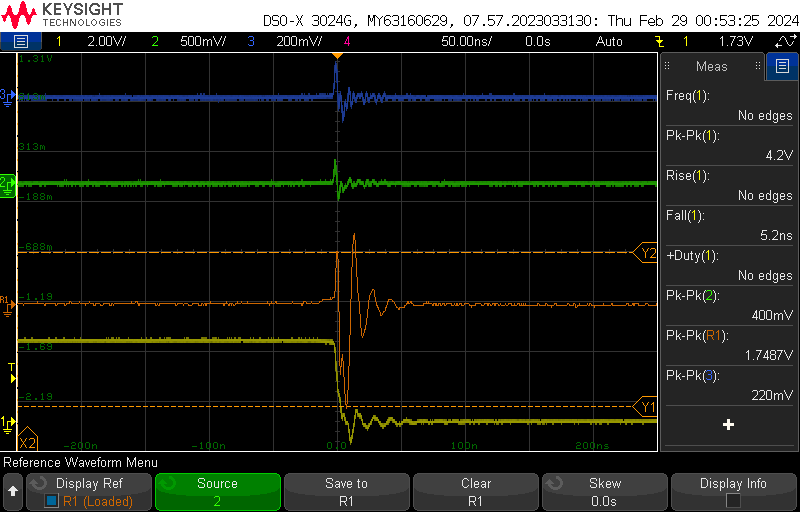
\includegraphics[scale=0.6]{figures/ql_falling}
		\caption{Quite Low on Falling Edge}
	
	\end{figure}

	\begin{figure}[H]
		\centering
		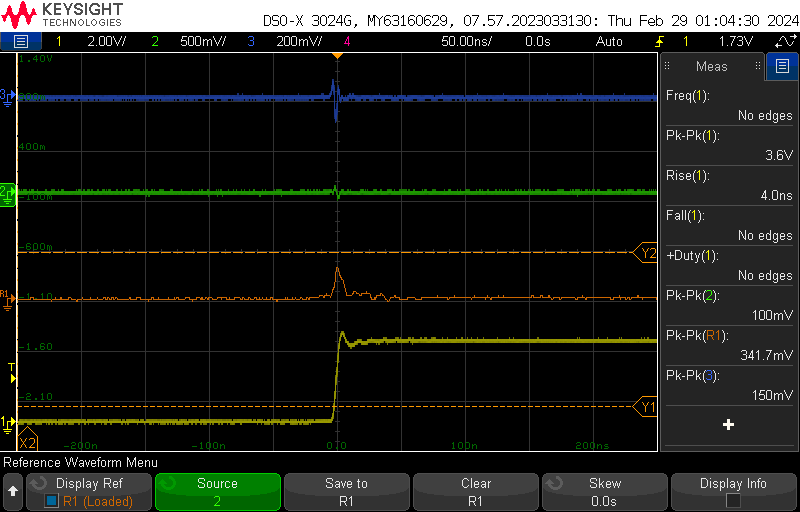
\includegraphics[scale=0.6]{figures/low_rising}
		\caption{Quite Low on Rising Edge}
	
	\end{figure}

	\textbf{Screenshot Explanation:} The screenshot shows all the Q\_lows from the board, Blue line represents Good layout, green line represents bad layout and orange line represents worst layout 
	
	we are getting noise level as 
	\begin{table}[H]
		\centering
		\begin{tabular}{c c c}
			\hline
			\textbf{Layout}  &  \textbf{Noise on Rising Edge} & \textbf{Noise on Falling edge}              \\\hline
			  &                                       \\
			Good Layout & 150 mV & 220 mV\\
			Bad layout & 100 mV & 400 mV \\
			Worst Layout& 340 mV & 1.7487 V        \\
			
			\hline\hline
		\end{tabular}
		\caption{Quite High noise on both edge}
	\end{table}

	We are expecting this behavior of getting less noise in rising edge as we know that in CMOS rising edge is slower than falling edge so fall time would be faster and we can expect to see that
	\item \textbf{Q\_hi Noise:}
	
	\textbf{Measurement:} Measure the peak-to-peak voltage of the noise observed on the Q\_hi test point using the cursors.

	\begin{figure}[H]
		\centering
		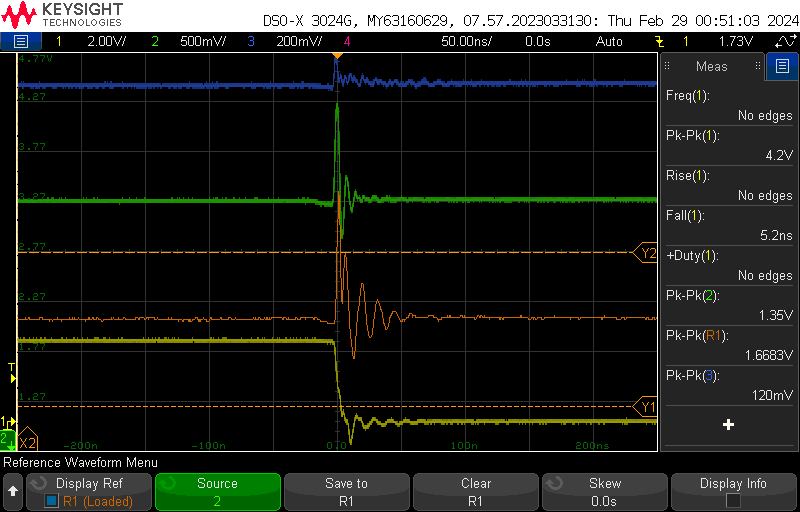
\includegraphics[scale=0.6]{figures/qh_falling}
		\caption{Quite High on Falling Edge}
	
	\end{figure}

	\begin{figure}[H]
		\centering
		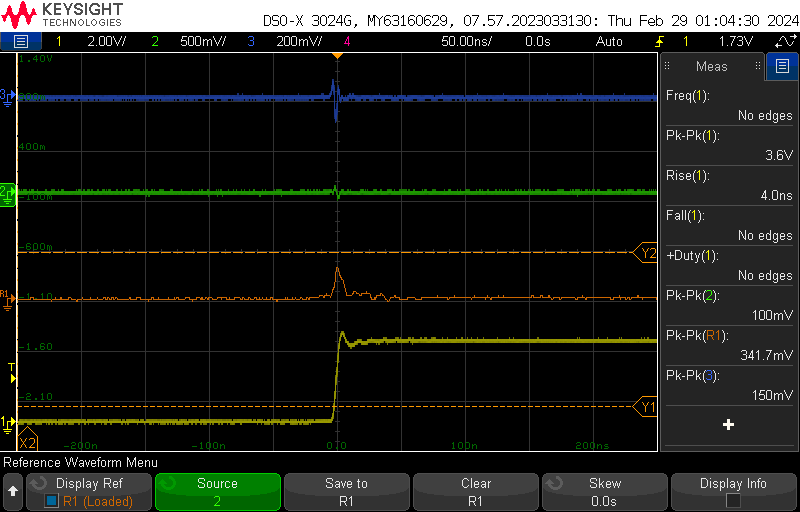
\includegraphics[scale=0.6]{figures/low_rising}
		\caption{Quite High on Rising Edge}
	
	\end{figure}

	\textbf{Screenshot Explanation:} The screenshot shows all the Q\_lows from the board, Blue line represents Good layout, green line represents bad layout and orange line represents worst layout 
	
	we are getting noise level as 
	\begin{table}[H]
		\centering
		\begin{tabular}{c c c}
			\hline
			\textbf{Layout}  &  \textbf{Noise on Rising Edge} & \textbf{Noise on Falling edge}              \\\hline
			  &                                       \\
			Good Layout &150 mV&120 mV\\
			Bad layout &120 mV&1.35 V\\
			Worst Layout&341.7 mV&1.6683 V         \\
			
			\hline\hline
		\end{tabular}
		\caption{Quite High noise on Both edge}
	\end{table}
	We are expecting this behavior of getting less noise in rising edge as we know that in CMOS rising edge is slower than falling edge so fall time would be faster and we can expect to see that

	\item \textbf{Power Rail Noise (5V and 3.3V):}

	\textbf{Measurement:} Zoom in on the 5V and 3.3V rail test points and measure any synchronous noise with the switching signal. Observe the peak-to-peak voltage of these noise spikes.

	\begin{figure}[H]
		\centering
		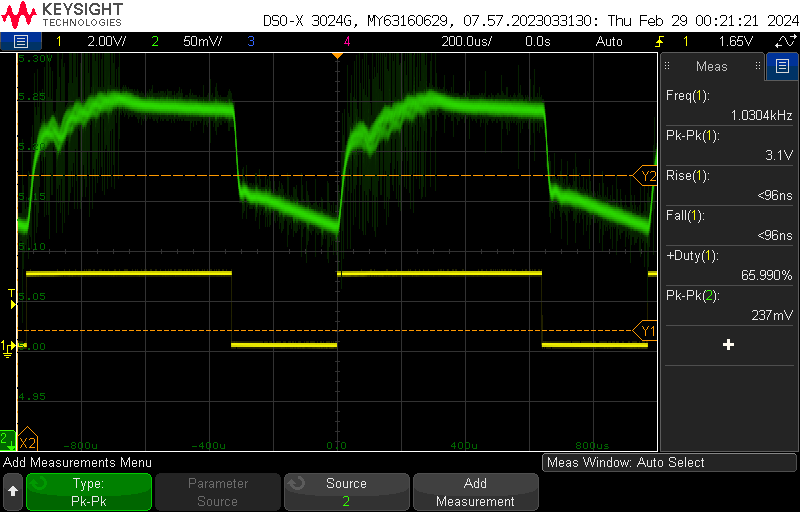
\includegraphics[scale=0.6]{figures/5v_switching_noise}
		\caption{5V switching noise}
	
	\end{figure}

	\begin{figure}[H]
		\centering
		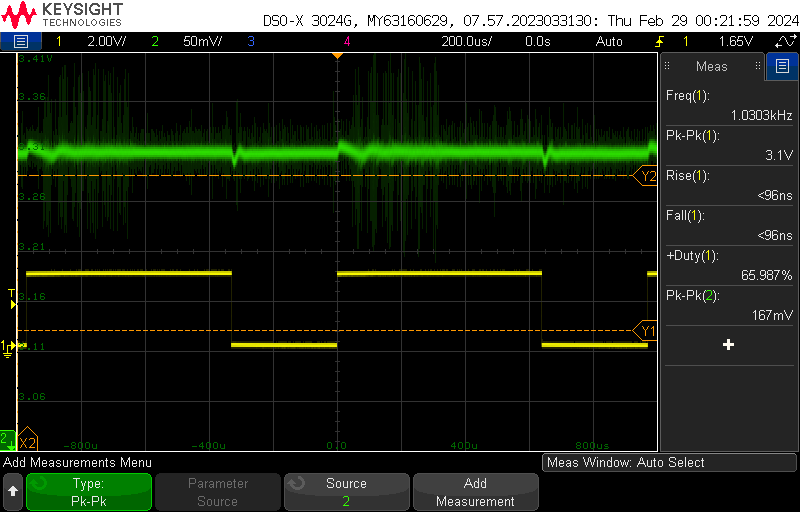
\includegraphics[scale=0.6]{figures/3v_switching_noise}
		\caption{3.3V switching noise}
	
	\end{figure}

	\textbf{Screenshot Explanation:}The screenshot show a zoomed-in view of the power rail voltage. Ideally, it should be a flat line representing the DC voltage level. but there might be spikes or dips in the voltage corresponding to switching events. 

	We can see that 5V rail has noise around 237mV peak to peak and 3.3V rail has around 167mV peak to peak.

\end{enumerate}

\textbf{Expected Observations:}

By comparing screenshots from different layouts, you should observe:

\begin{enumerate}
	\item Lower peak-to-peak noise voltage on Q\_low and Q\_hi in the good layout compared to bad layouts.
	\item From the Calculations section we can see 87\% decrease in the noise from Worst layout to good layout
\end{enumerate}




\section{Learnings and Observation}\

\textbf{Learning Outcomes:}

This experiment provided valuable insights into the critical role of PCB layout in controlling switching noise:

\begin{enumerate}
	\item Impact of Layout Practices: The experiment demonstrated that proper layout techniques, such as utilizing a continuous return path and placing decoupling capacitors close to ICs, significantly reduce switching noise compared to layouts lacking these features.

	\item Practical Design Considerations: The experiment emphasized the practical considerations for future PCB layouts, including prioritizing a continuous return path, strategically placing decoupling capacitors, and minimizing trace lengths.
\end{enumerate}





\section{Conclusion}



This experiment successfully investigated the impact of PCB layout on switching noise. The measurements confirmed that the good layout, featuring a return path and close decoupling capacitors, exhibited significantly lower noise levels compared to the bad layouts. This supports the theoretical understanding of how layout choices influence current flow, voltage stability, and ultimately, signal integrity.

\textbf{Key observations:}
\begin{itemize}
	\item Reduced Q\_low and Q\_hi noise: The good layout displayed 87\% lower noise compared to the worst layout, highlighting the effectiveness of proper layout practices.
	\item Minimal power rail noise: The good layout exhibited minimal noise on the 5V and 3.3V rails, demonstrating the effectiveness of the return path and decoupling capacitors in mitigating noise propagation.
\end{itemize}





\pagebreak
\hrule
\hrule
\hrule






%---------------------------------------------------------------------------
\end{document}
-
